\documentclass{beamer}
\usepackage[utf8]{inputenc}
\usetheme{default}

\usepackage{tikz}
\usetikzlibrary{decorations.pathreplacing}
\usepackage{subfigure}
\usepackage{gitdags}

\usepackage{csquotes}
\usepackage[style=authortitle,backend=bibtex]{biblatex}
\bibliography{slides}

\usepackage{listings}

\newtheorem{defn}{Définition}

\title{Fouine comme moteur du progrès des méthodes de gestion de projet collaboratif en milieu normalien : une retrospective comparative de Février 2021 à nos jours}
\author{Maxime Cautrès \and Pierre Goutagny}
\date{21 Floréal An CCXXIX}

\begin{document}
\maketitle

\begin{frame}
\frametitle{Définitions}

\pause
\begin{defn}[Fouine]\end{defn}
\pause
\begin{defn}[Git]\end{defn}
\end{frame}

\begin{frame}
\frametitle{Un projet, en somme, c'est comme un grand terrier\ldots}
Saurez-vous trouver la différence subtile entre ces deux photos ?
\begin{figure}
\centering
\subfigure[\onslide<2->{entrée Nord}] {
    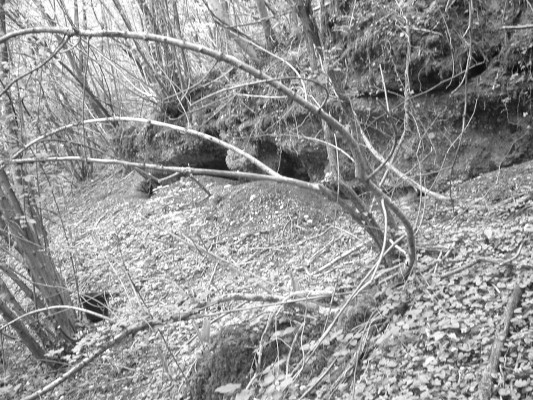
\includegraphics[scale=.4]{terrierN}
}
\subfigure[\onslide<2->{entrée Nord-Est}] {
    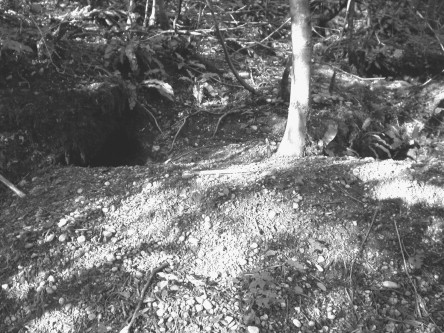
\includegraphics[scale=.45]{terrierNE}
}
\onslide<2->{\caption{un terrier, deux entrées}}
\end{figure}
\only<3>{Pour explorer un grand terrier (plus d'un hectare\autocite{MALLYE2008187}), on peut entrer par plusieurs trous.}
\end{frame}

\begin{frame}
\frametitle{Ah non en fait l'analogie c'est avec un arbre, pas un terrier}

\only<1>{
    \begin{figure}
    \centering
        \begin{tikzpicture}[scale=.8, every node/.style={scale=.7}]
        % Commit DAG
        \gitDAG[grow left sep = 1em]{
            e633469 -- {
                8c06958 -- 10e05c9 -- { 41c6d8b -- bc0e2b3 -- {
                    9fac073 -- 6fd6a94 -- b332dd2,
                            6824623 -- 9fac073,
                },
                        d62129a -- 6824623 -- 9fac073,
                        6486be3 -- a148b0f -- 6095c48 -- c1a7235 -- 9b28e51 -- "$\cdots$" -- b332dd2,
                },
                        5b93933 -- {
                            ed2d0c9 -- bc0e2b3,
                            10e05c9,
                        },
                        b490ade -- {
                            6fd6a94,
                            9f28e51,
                        },
            }
        };
    \end{tikzpicture}
    \caption{sans les branches}
    \end{figure}
}
\only<2>{
    \begin{figure}
    \centering
        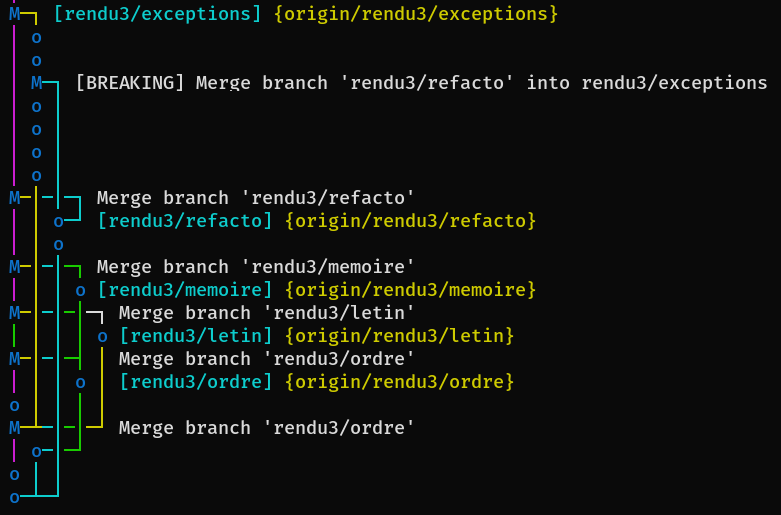
\includegraphics[scale=.35]{branches_joli_edit}
    \caption{avec des branches}
    \end{figure}

}
\end{frame}

\begin{frame}
\frametitle{Les avantages totalement objectifs à utiliser des branches}
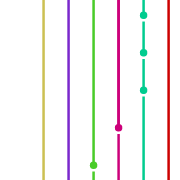
\includegraphics[scale=.5]{paralleles}<2>

\includegraphics[scale=.3]{stats}<3>
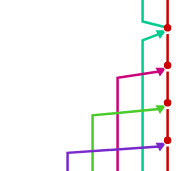
\includegraphics[scale=.3]{merge}<4>
\begin{itemize}
    \item<2-> paralléliser
    \item<3-> fragmenter les fonctionnalités
    \item<4-> la satisfaction des jolis schémas
\end{itemize}
\end{frame}

\begin{frame}[fragile]
\frametitle{Inconvénients}
\pause
Parfois c'est difficile à utiliser\pause, mais \ldots
\begin{verbatim}
man git branch
\end{verbatim}
\pause
\begin{verbatim}
man git merge
\end{verbatim}
\pause
\begin{verbatim}
man git
\end{verbatim}
\pause
\begin{verbatim}
man man
\end{verbatim}
\end{frame}

\begin{frame}
\frametitle{Références}
\printbibliography
\end{frame}

\begin{frame}
\flushright des questions ?

\includegraphics[scale=.48]{fin}<1,3>
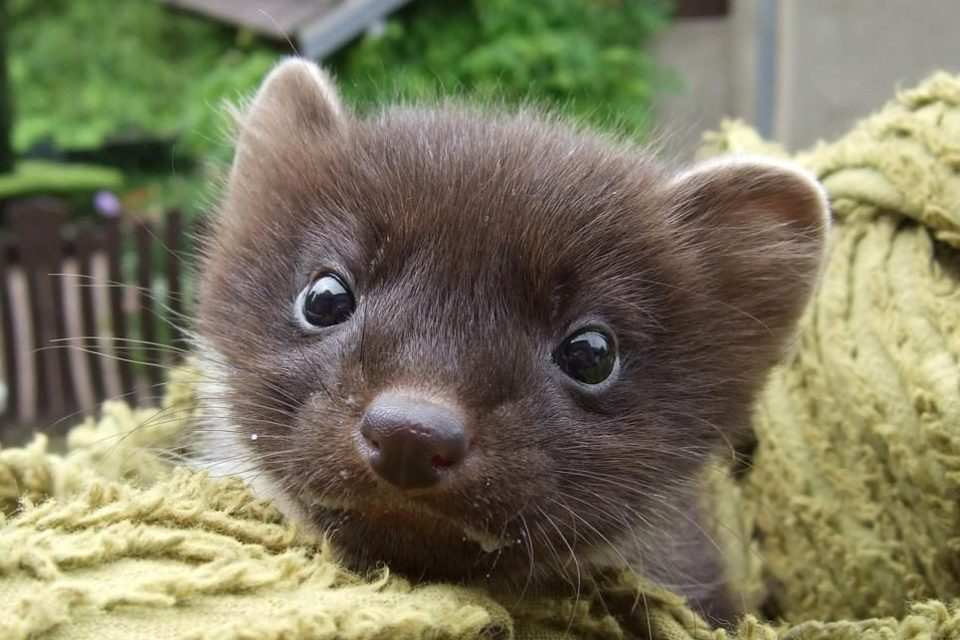
\includegraphics[scale=.4]{fouinefin}<2>
\end{frame}

\end{document}

